\documentclass{article}
\usepackage[utf8]{inputenc}
\usepackage{graphicx}

\author{Bijan Varjavand}
\title{LabNotebook}
\date{February 28, 2017}

\begin{document}

\maketitle

\section{Objectives}

The goal this lab was to measure capacitance values using an LCR meter, while changing properties of the material we were measuring. This would hopefully result in interesting data.

\section{Setup}

LCR meters and the materials were provided by the lab. We were also given copper tape, and RO and tap water were both provided.

\subsection{Materials}

We used firebrick.

\subsection{Tools}

We used LCR meters and wires along with alligator clips.

\section{Procedure}

We took a single sample of firebrick and measured thickness. Attaching three differently sized copper pieces to one side, and covering the other side with copper tape. We then measured capacitance and dissipation factor at three different frequencies. We did this to the same sample after submerging it in RO water, and then regular water.

\section{Results}

An example of the trends we found from these measurements are shown below.

\begin{figure}[h!]
\centering
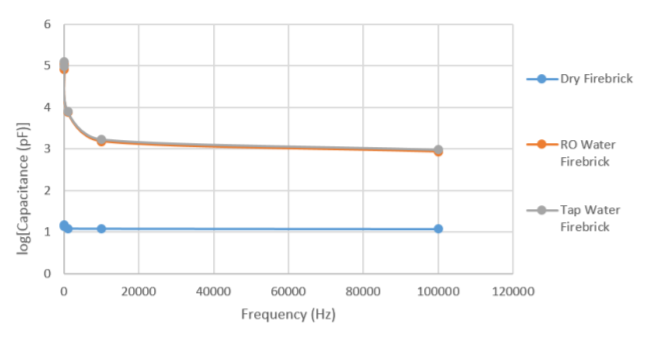
\includegraphics[scale=0.8]{fire.png}
\end{figure}

\section{Observations}

These results elucidates the relationship between capacitance and the existence of charge carriers in the material. This is shown by the greatly increased capacitance when we add water, which has natural hydronium and hydroxide ions.

\end{document}